\begin{enumerate}
    \item the \verb|whois| command shows information about who has registered the domain name specified.
    \begin{figure}[H]
        \centering
        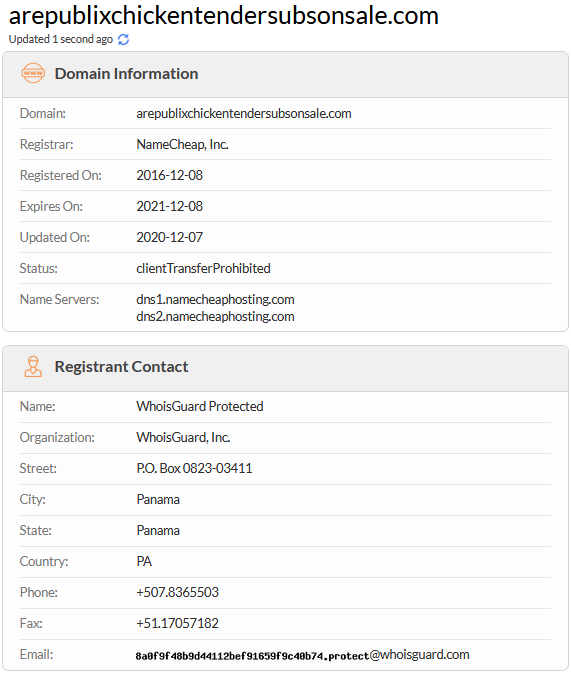
\includegraphics[width=\linewidth]{figures/whois1.png}
    \end{figure}
    \begin{figure}[H]
        \centering
        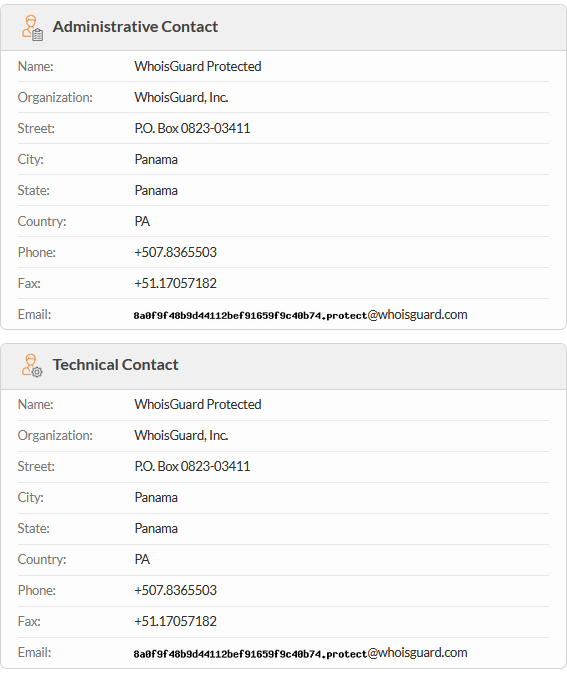
\includegraphics[width=\linewidth]{figures/whois2.png}
    \end{figure}
    I ran the command via the Windows command prompt but there were to many lines to input them cleanly into the report so I went to \url{https://www.whois.com/whois/arepublixchickentendersubsonsale.com} and was given this information.

    The website \url{www.arepublixchickentendersubsonsale.com} is hosted by NameCheap which uses WhoisGuard to handle whois commands.
    \item The \verb|nslookup| command is used to query domain name servers for information about parts of the DNS namespace or individual hosts.
    Here we use it to find the mail exchange server.
    \begin{figure}[H]
        \centering
        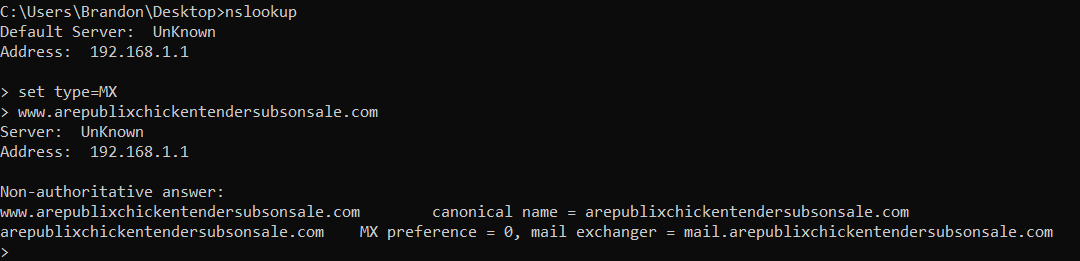
\includegraphics[width=\linewidth]{figures/nslookup1.png}
    \end{figure}
\end{enumerate}

In this lab I learned how to use the \verb|whois| and \verb|nslookup| tools.
\verb|Whois| is used to gather information about a domains registration and the contacts associated with the domains registrars.
\verb|Nslookup| is used to get information about more specific parts of a domains namespace, or individual hosts such as the mail exchange server or default servers.